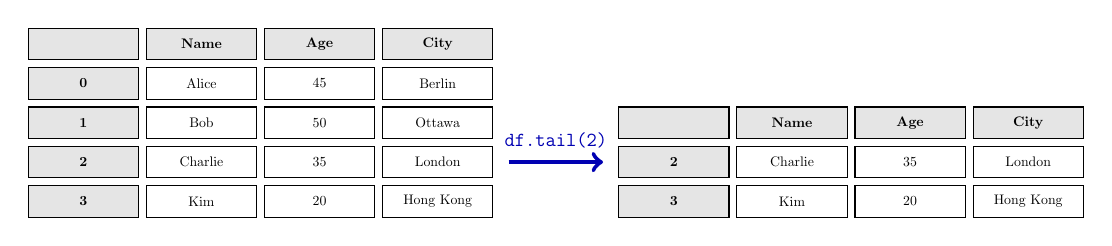
\begin{tikzpicture}[
    scale=0.5, 
    transform shape,
    cell/.style={
        draw,
        minimum width=2.8cm,
        minimum height=0.8cm,
        align=center
    },
    header/.style={
        cell,
        fill=gray!20,
        font=\bfseries
    }
]
    % --- Headers ---
    \node[header] (h0) at (0,0) {};
    \node[header] (h1) at (3,0) {Name};
    \node[header] (h2) at (6,0) {Age};
    \node[header] (h3) at (9,0) {City};

    % --- Row 0 ---
    \node[header] at (0,-1) {0};
    \node[cell] at (3,-1) {Alice};
    \node[cell] at (6,-1) {45};
    \node[cell] at (9,-1) {Berlin};

    % --- Row 1 ---
    \node[header] at (0,-2) {1};
    \node[cell] at (3,-2) {Bob};
    \node[cell] at (6,-2) {50};
    \node[cell] at (9,-2) {Ottawa};

    % --- Row 2 ---
    \node[header] at (0,-3) {2};
    \node[cell] at (3,-3) {Charlie};
    \node[cell] at (6,-3) {35};
    \node[cell] at (9,-3) {London};

    % --- Row 3 ---
    \node[header] at (0,-4) {3};
    \node[cell] at (3,-4) {Kim};
    \node[cell] at (6,-4) {20};
    \node[cell] at (9,-4) {Hong Kong};

    \draw[->, ultra thick, blue!70!black]
        (10.8,-3)
        to[out=0,in=180]
        node[midway, above=6pt, font=\ttfamily\Large] {df.tail(2)}
        (13.2,-3);

    % Result of df.tail(2)
    \node[header] at (15,-2) {};
    \node[header] at (18,-2) {Name};
    \node[header] at (21,-2) {Age};
    \node[header] at (24,-2) {City};

    % --- Row 2 ---
    \node[header] at (15,-3) {2};
    \node[cell] at (18,-3) {Charlie};
    \node[cell] at (21,-3) {35};
    \node[cell] at (24,-3) {London};

    % --- Row 3 ---
    \node[header] at (15,-4) {3};
    \node[cell] at (18,-4) {Kim};
    \node[cell] at (21,-4) {20};
    \node[cell] at (24,-4) {Hong Kong};
\end{tikzpicture}
